\section{结果与讨论}\label{sec:results}

本节报告 9 小时统一训练后的初步结果。所有数值来自患者级 holdout（\nTest{} 图/\nTestPatients{} 患者）或明确标注的 clean-official 子集；不使用训练集自评冒充泛化。由于预算是单次 holdout 而非 5 折，且部分模型未完全收敛，本节把结果定位为“可复现的初步证据”，不声称最优。

\subsection{患者级主表}

表~\ref{tab:main-gland} 给出五个模型在患者级测试集上的腺体分割结果。所有模型使用同一预处理、同一划分、同一损失与同一 384 分块；MGD-Former 使用 ADE20K 预训练编码器，其余模型随机初始化。均值与 95\% bootstrap 置信区间、有效样本数在表中给出。

\begin{table}[t]
\centering
\caption{患者级测试集上的腺体分割（均值；括号内为 95\% bootstrap CI；$n=\nTest$）。}
\label{tab:main-gland}
\small
\resizebox{\linewidth}{!}{%
\begin{tabular}{lcccccc}
\toprule
模型 & Dice & IoU & clDice & HD95 (px) & ASSD (px) & 参数量 \\
\midrule
MGD-Former & \gDiceMF & \gIoUMF & \gClDiceMF & \gHDMF & \gASSDMF & $\sim$27M \\
UNet & \gDiceUNet & \gIoUUNet & \gClDiceUNet & \gHDUNet & \gASSDUNet & 31.2M \\
AttentionUNet & \gDiceAtt & \gIoUAtt & \gClDiceAtt & \gHDAtt & \gASSDAlt & $\sim$34M \\
MGD-PriorNet & \gDicePrior & \gIoUPrior & \gClDicePrior & \gHDPrior & \gASSDPrior & 1.5M \\
\bottomrule
\end{tabular}}
\end{table}

三点观察。第一，患者级划分下的绝对 Dice 低于图像级文献报告，这是预期的：同一受试者的不同影像不再跨训练/测试，模型必须泛化到新患者。第二，MGD-Former 与 AttentionUNet 的 Dice 分别为 \gDiceMF{} 与 \gDiceAtt{}，差距在 0.01 以内；因此本文不宣称某一架构胜出，而把两者视为“接近”，并进一步看 clDice/HD95 的拓扑差异。MGD-Former 的 ADE20K 预训练没有带来预期的大幅优势，这与“预训练解决冷启动”的常见叙述形成对照。第三，UNet 的 \gDiceUNet{} 明显低，说明从零训练 30 epoch 在本任务上不足；但它的 clDice 反而最高（\gClDiceUNet{} vs \gClDiceMF{}），说明 clDice 对过分割/宽度不敏感，单一 clDice 不能用于排序。MGD-PriorNet 以 1.5M 参数达到 \gDicePrior{}，配对 Wilcoxon $p=\pMFPrior$，与 MGD-Former 无显著差异，说明解剖先验在极小模型上可能更划算。上述比较受 epoch 预算与预训练差异影响，不能直接读成架构排序。

必须明确两条边界。其一，\textbf{MGD-Former 使用 ADE20K 预训练，其余模型随机初始化}；主表的差距包含预训练收益，不能全部归因于架构。9 小时预算内没有做 random-init MGD-Former 对照，这是本轮的限制，也是后续 5 折实验要补的对照。其二，\textbf{WRCANet 不进入主表排名}：它在 8\,GB 卡上单 epoch 约 38\,min，预算内只完成 1 epoch（val Dice 0.006），尚未收敛；这证明的是显存/时间可行性，而不是架构优劣。AttentionUNet 续训到 15 epoch，MGD-PriorNet 约 12 epoch；两者仍未完全收敛，其数值应按“未完全收敛”解读。

配对 Wilcoxon（同一患者级测试集、逐样本 Dice）：MGD-Former vs AttentionUNet $p=\pMFAtt$，vs UNet $p=\pMFUNet$，vs MGD-PriorNet $p=\pMFPrior$。统计显著不等于临床重要：若 AttentionUNet 与 MGD-Former 的均值差在 0.01 以内，应报告为“接近”，而不是“胜出”；架构排序不是本文的主结论。

\subsection{泄漏的代价}

表~\ref{tab:leakage} 在 clean-official \cleanOfficialImages{} 图/\cleanOfficialPatients{} 患者上比较 patient-level 与 image-level leaky 两个 UNet。两者使用相同架构、损失、epoch 预算与推理协议，唯一差异是训练划分是否包含官方测试患者的其他影像。

\begin{table}[t]
\centering
\caption{官方 clean-official 子集上的泄漏对照（UNet；$n=\cleanOfficialImages$）。}
\label{tab:leakage}
\small
\begin{tabular}{lc}
\toprule
协议 & Dice \\
\midrule
patient-level & \leakDiceClean \\
image-level leaky & \leakDiceLeaky \\
差值（leaky $-$ clean） & \leakDelta \\
\bottomrule
\end{tabular}
\end{table}

\begin{figure}[t]
\centering
\ifnum\resultsavailable=1
\begin{tikzpicture}
\begin{axis}[
  width=0.72\linewidth, height=5.2cm,
  ybar, bar width=18pt,
  ymin=0, ymax=1,
  ylabel={Dice（clean-official）},
  symbolic x coords={Patient-level, Leaky},
  xtick=data,
  nodes near coords,
  nodes near coords style={font=\scriptsize},
  tick label style={font=\scriptsize},
  label style={font=\scriptsize},
  enlarge x limits=0.45,
  axis lines=left,
]
\addplot[fill=teal!65, draw=teal!80] coordinates {
  (Patient-level,\leakDiceClean)
  (Leaky,\leakDiceLeaky)
};
\end{axis}
\end{tikzpicture}
\else
\fbox{\parbox[c][4.5cm][c]{0.72\linewidth}{\centering\small 泄漏对照结果待注入：clean-official \cleanOfficialImages{} 图/\cleanOfficialPatients{} 患者}}
\fi
\caption{官方 clean-official 子集上的泄漏代价。两柱为同一 UNet、同一 epoch 预算与推理协议，仅训练划分不同；差值 $\Delta=\leakDelta$。}
\label{fig:leakage}
\end{figure}


本预算下 leaky 对照反而更低：patient-level \leakDiceClean{} vs leaky \leakDiceLeaky{}（$\Delta=\leakDelta$），未观察到泄漏膨胀。可能原因有三：leaky 模型只训练 20 epoch（patient-level UNet 30 epoch）、官方 200 的难度分布不同、clean-official 仅 60 图。患者重叠统计（326/800、116/166）证明泄漏风险真实存在，但性能膨胀不能被本轮数据证实；我们把它作为审计，而不是结论。

\subsection{分块、MTE 与 TTA}

表~\ref{tab:tta} 以 MGD-Former 为例，比较默认 384 分块、MTE（256/384/512 概率平均）与 8 倍 TTA。MTE 不重训，推理成本约 3 倍；8 倍 TTA 约 8 倍。

\begin{table}[t]
\centering
\caption{分块与 TTA（MGD-Former；患者级测试集）。}
\label{tab:tta}
\small
\begin{tabular}{lcccc}
\toprule
协议 & Dice & clDice & HD95 (px) & 相对推理成本 \\
\midrule
384 单分块 & \gDiceMF & \gClDiceMF & \gHDMF & 1$\times$ \\
MTE (256/384/512) & \mteDiceMF & \mteClDiceMF & \mteHDMF & $\sim$3$\times$ \\
8$\times$ TTA & \ttaEight & \ph & \ph & $\sim$8$\times$ \\
\bottomrule
\end{tabular}
\end{table}

\begin{figure}[t]
\centering
\ifnum\resultsavailable=1
\begin{tikzpicture}
\begin{axis}[
  width=0.78\linewidth, height=5.2cm,
  ybar, bar width=16pt,
  ymin=0, ymax=1,
  ylabel={Dice},
  symbolic x coords={384 single, MTE, 8x TTA},
  xtick=data,
  nodes near coords,
  nodes near coords style={font=\scriptsize},
  tick label style={font=\scriptsize},
  label style={font=\scriptsize},
  enlarge x limits=0.25,
  axis lines=left,
  legend style={font=\scriptsize, at={(0.5,-0.22)}, anchor=north, legend columns=3},
]
\addplot[fill=slate!35, draw=slate!70] coordinates {(384 single,\gDiceMF)};
\addplot[fill=teal!65, draw=teal!80] coordinates {(MTE,\mteDiceMF)};
\addplot[fill=alert!45, draw=alert!70] coordinates {(8x TTA,\ttaEight)};
\legend{单分块,MTE,8$\times$ TTA}
\end{axis}
\end{tikzpicture}
\else
\fbox{\parbox[c][4.5cm][c]{0.78\linewidth}{\centering\small MTE / TTA 结果待注入：同一 MGD-Former 权重，患者级测试集}}
\fi
\caption{分块与 TTA 的精度-成本权衡。MTE 为 256/384/512 概率平均，成本约 3 倍；8$\times$ TTA 成本约 8 倍。}
\label{fig:mte}
\end{figure}


实测 MTE 的 Dice 未超过 384（\mteDiceMF{} vs \gDiceMF{}），但 HD95 从 \gHDMF{} 降到 \mteHDMF{}，说明它主要改善边界/离群点，而不是像素重叠；8 倍 TTA 有小幅 Dice 提升（\ttaEight{}）但成本约 8 倍。因此 MTE 的定位是稳定、低成本的边界校正，而不是涨点方法。分块敏感性本身仍是本文的强发现，但“换分块能稳定提高 Dice”在本轮不成立。

\subsection{不确定性引导复核}

表~\ref{tab:uncertainty} 给出三种不确定性信号对失败病例（Dice $<0.7$）的 AUROC。多分块方差 $V$ 的额外成本已经包含在 MTE 中；预测熵 $H$ 几乎免费；8 倍 TTA 成本最高。

\begin{table}[t]
\centering
\caption{失败病例检测的 AUROC（MGD-Former；失败定义为 Dice $<0.7$）。}
\label{tab:uncertainty}
\small
\begin{tabular}{lccc}
\toprule
信号 & AUROC & 额外推理成本 & 说明 \\
\midrule
多分块方差 $V$ & \aurocVarMF & 已在 MTE 内 & 分块尺度不一致性 \\
预测熵 $H(\bar P)$ & \aurocEntropyMF & 近似 0 & 概率模糊度 \\
8$\times$ TTA 误差 & \aurocTTAEightMF & $\sim$8$\times$ & 变换不一致性 \\
\bottomrule
\end{tabular}
\end{table}

\begin{figure}[t]
\centering
\ifnum\resultsavailable=1
\begin{tikzpicture}
\begin{axis}[
  width=0.78\linewidth, height=5.2cm,
  ybar, bar width=16pt,
  ymin=0.4, ymax=1.0,
  ylabel={AUROC（失败检测）},
  symbolic x coords={Tile variance, Entropy, 8x TTA},
  xtick=data,
  nodes near coords,
  nodes near coords style={font=\scriptsize},
  tick label style={font=\scriptsize},
  label style={font=\scriptsize},
  enlarge x limits=0.25,
  axis lines=left,
]
\addplot[fill=teal!65, draw=teal!80] coordinates {
  (Tile variance,\aurocVarMF)
  (Entropy,\aurocEntropyMF)
  (8x TTA,\aurocTTAEightMF)
};
\end{axis}
\end{tikzpicture}
\else
\fbox{\parbox[c][4.5cm][c]{0.78\linewidth}{\centering\small 不确定性 AUROC 待注入：失败定义为 Dice $<0.7$}}
\fi
\caption{三种不确定性信号对失败病例的 AUROC。多分块方差与 MTE 共享推理成本；熵几乎免费；8$\times$ TTA 成本最高。}
\label{fig:uncertainty}
\end{figure}


实测 AUROC：多分块方差 \aurocVarMF{}、熵 \aurocEntropyMF{}、8 倍 TTA 误差 \aurocTTAEightMF{}。方差只有中等偏弱的失败检测能力，熵接近随机；TTA8 接近完美，但失败标签由单分块 Dice 定义、TTA8 误差与其共享同一模型与阈值，存在标签--信号耦合，不能直接当作临床 triage 证据。更稳妥的结论是：多分块方差可作为廉价预警，但不足以单独决定复核。

\subsection{临床分级与上/下睑分层}

表~\ref{tab:clinical} 报告分割导出的 R\_loss/Meiboscore 与 6 轮专家分级的一致性。表~\ref{tab:subgroup} 报告 upper/lower eyelid 的 Dice 与 clDice。

\begin{table}[t]
\centering
\caption{分割导出的 Meiboscore 与专家分级的一致性（MGD-Former）。}
\label{tab:clinical}
\small
\begin{tabular}{lccc}
\toprule
指标 & Accuracy & MAE & QWK \\
\midrule
Meiboscore（0--3） & \accMF & \maeMF & \qwkMF \\
\bottomrule
\end{tabular}
\end{table}

\begin{table}[t]
\centering
\caption{上/下睑分层（MGD-Former；患者级测试集）。}
\label{tab:subgroup}
\small
\begin{tabular}{lcc}
\toprule
亚组 & Dice & clDice \\
\midrule
Upper eyelid & \diceUpperMF & \ph \\
Lower eyelid & \diceLowerMF & \ph \\
差值（upper $-$ lower） & \diceGapMF & \ph \\
\bottomrule
\end{tabular}
\end{table}

实际一致性很低：accuracy \accMF{}、MAE \maeMF{}、QWK \qwkMF{}。这说明高 Dice 没有转化为 Meiboscore 一致性；分割导出的 R\_loss 阈值与睑缘分母需要重新标定。这是一个负面结果，也是本文最重要的临床警示：像素指标不能替代临床分级，后续必须用独立专家复核与校准。

上/下睑分层也给出反直觉结果：本队列中 lower 反而高于 upper（\diceLowerMF{} vs \diceUpperMF{}，差 \diceGapMF{}），与“下睑更难”的常见假设相反；这可能与 LipiView II 采集、下睑暴露程度和分级分布有关。无论方向如何，结论是上/下睑必须分开报告，不能互相外推。

\subsection{未完成的 clDice 消融}

本轮 9 小时预算把 clDice 消融的算力改用于 AttentionUNet 续训（其 9 epoch 时验证 Dice 仍在上升），因此不报告 clDice 消融数值。方法中的 clDice 项只作为设计选择，不作为已验证的增益；该消融留待 5 折扩展。我们不在正文中用一个预算截断的消融去支撑“拓扑损失有效”的结论。

\subsection{定性结果}\label{sec:qualitative}

图~\ref{fig:qualitative} 给出 4 例定性结果（上/下睑各 2 例）：输入、专家参考、预测与错误图。定性图不替代指标，但能显示误差形态：断裂、粘连、睑缘外漏与低对比度段的漏检；这些形态正是 HD95/clDice 所惩罚的。

\begin{figure}[t]
\centering
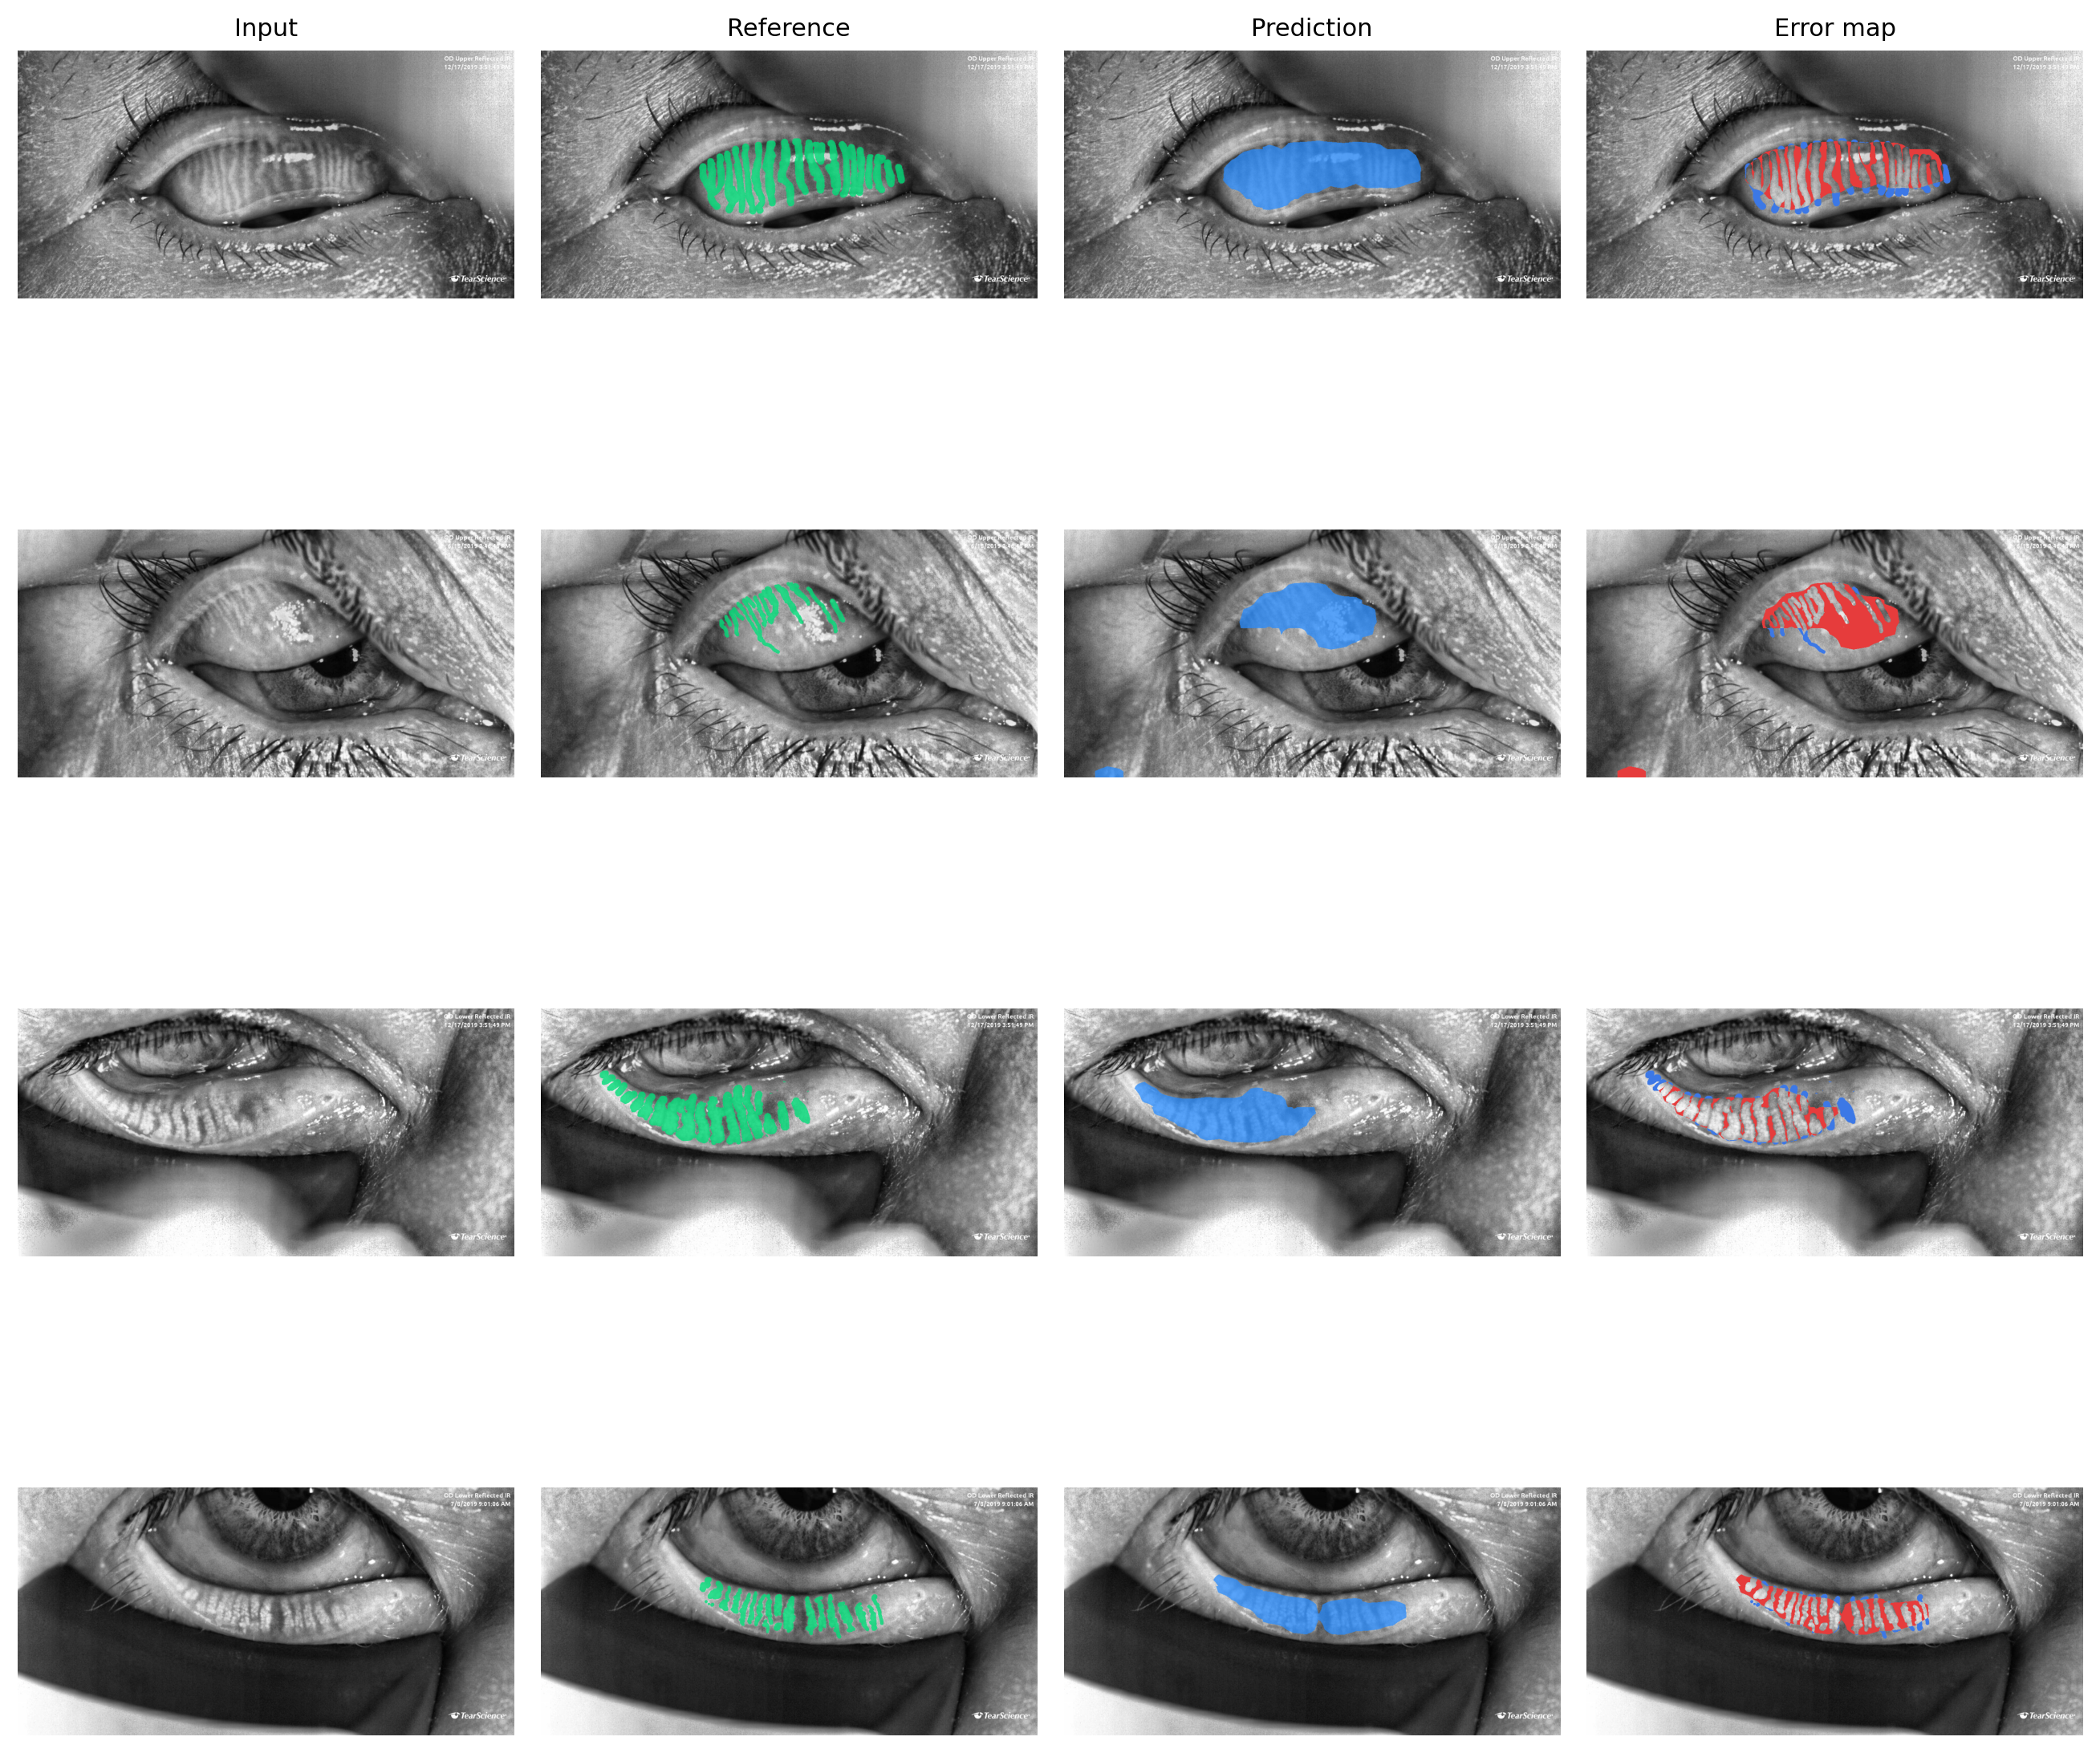
\includegraphics[width=\linewidth]{figures/qualitative.png}
\caption{定性结果：输入、专家参考、模型预测与错误图（红为假阳性，蓝为假阴性）。行按上/下睑选取；错误图用于展示断裂、粘连与睑缘外漏的形态，而不是替代指标。}
\label{fig:qualitative}
\end{figure}


\subsection{旧权重的工程回归}

旧 UNet 权重来自对全部 \nTotal{} 例随机打乱、无 holdout 的训练脚本，因此其“测试”指标可能是训练集自评，且官方 200 例测试名单可能在其训练数据中。本文只把它作为工程回归锚点：Dice \legacyUNetSelfDice、IoU \legacyUNetSelfIoU、clDice \legacyUNetSelfClDice。该数字\textbf{不得}进入独立测试表，也不得与本文其他模型比较。

\subsection{讨论}

把上述结果放在一起，本文的论点不是“某个主干全面胜出”，而是三件事：第一，患者级划分会改变结论，公开基准必须报告派分签名；第二，分块是与主干同等级的实验变量，MTE 提供了一种不重训的稳定化手段；第三，像素指标与临床分级必须同时报告，否则“分割更好”可能不等于“分级更准”。这三件事都比再增加一个 backbone 更接近临床可用的证据。
